% Actualization Chain Diagram — Organized by Completed Actualities
% with Motion and Time as aspects
% Compile with: pdflatex (requires tikz, amsmath)

\documentclass[border=12pt,tikz]{standalone}
\usepackage[T1]{fontenc}
\usepackage{amsmath}
\usepackage{tikz}
\usetikzlibrary{
  arrows.meta,
  positioning,
  calc,
  decorations.pathreplacing,
  fit,
  backgrounds,
  shapes.geometric
}

\definecolor{actuality}{RGB}{30,60,120}
\definecolor{motion}{RGB}{140,40,40}
\definecolor{timecolor}{RGB}{60,120,60}
\definecolor{moodcolor}{RGB}{160,120,40}
\definecolor{perceptual}{RGB}{225,237,252}
\definecolor{cognitive}{RGB}{252,240,225}
\definecolor{loopcolor}{RGB}{100,100,100}

\begin{document}
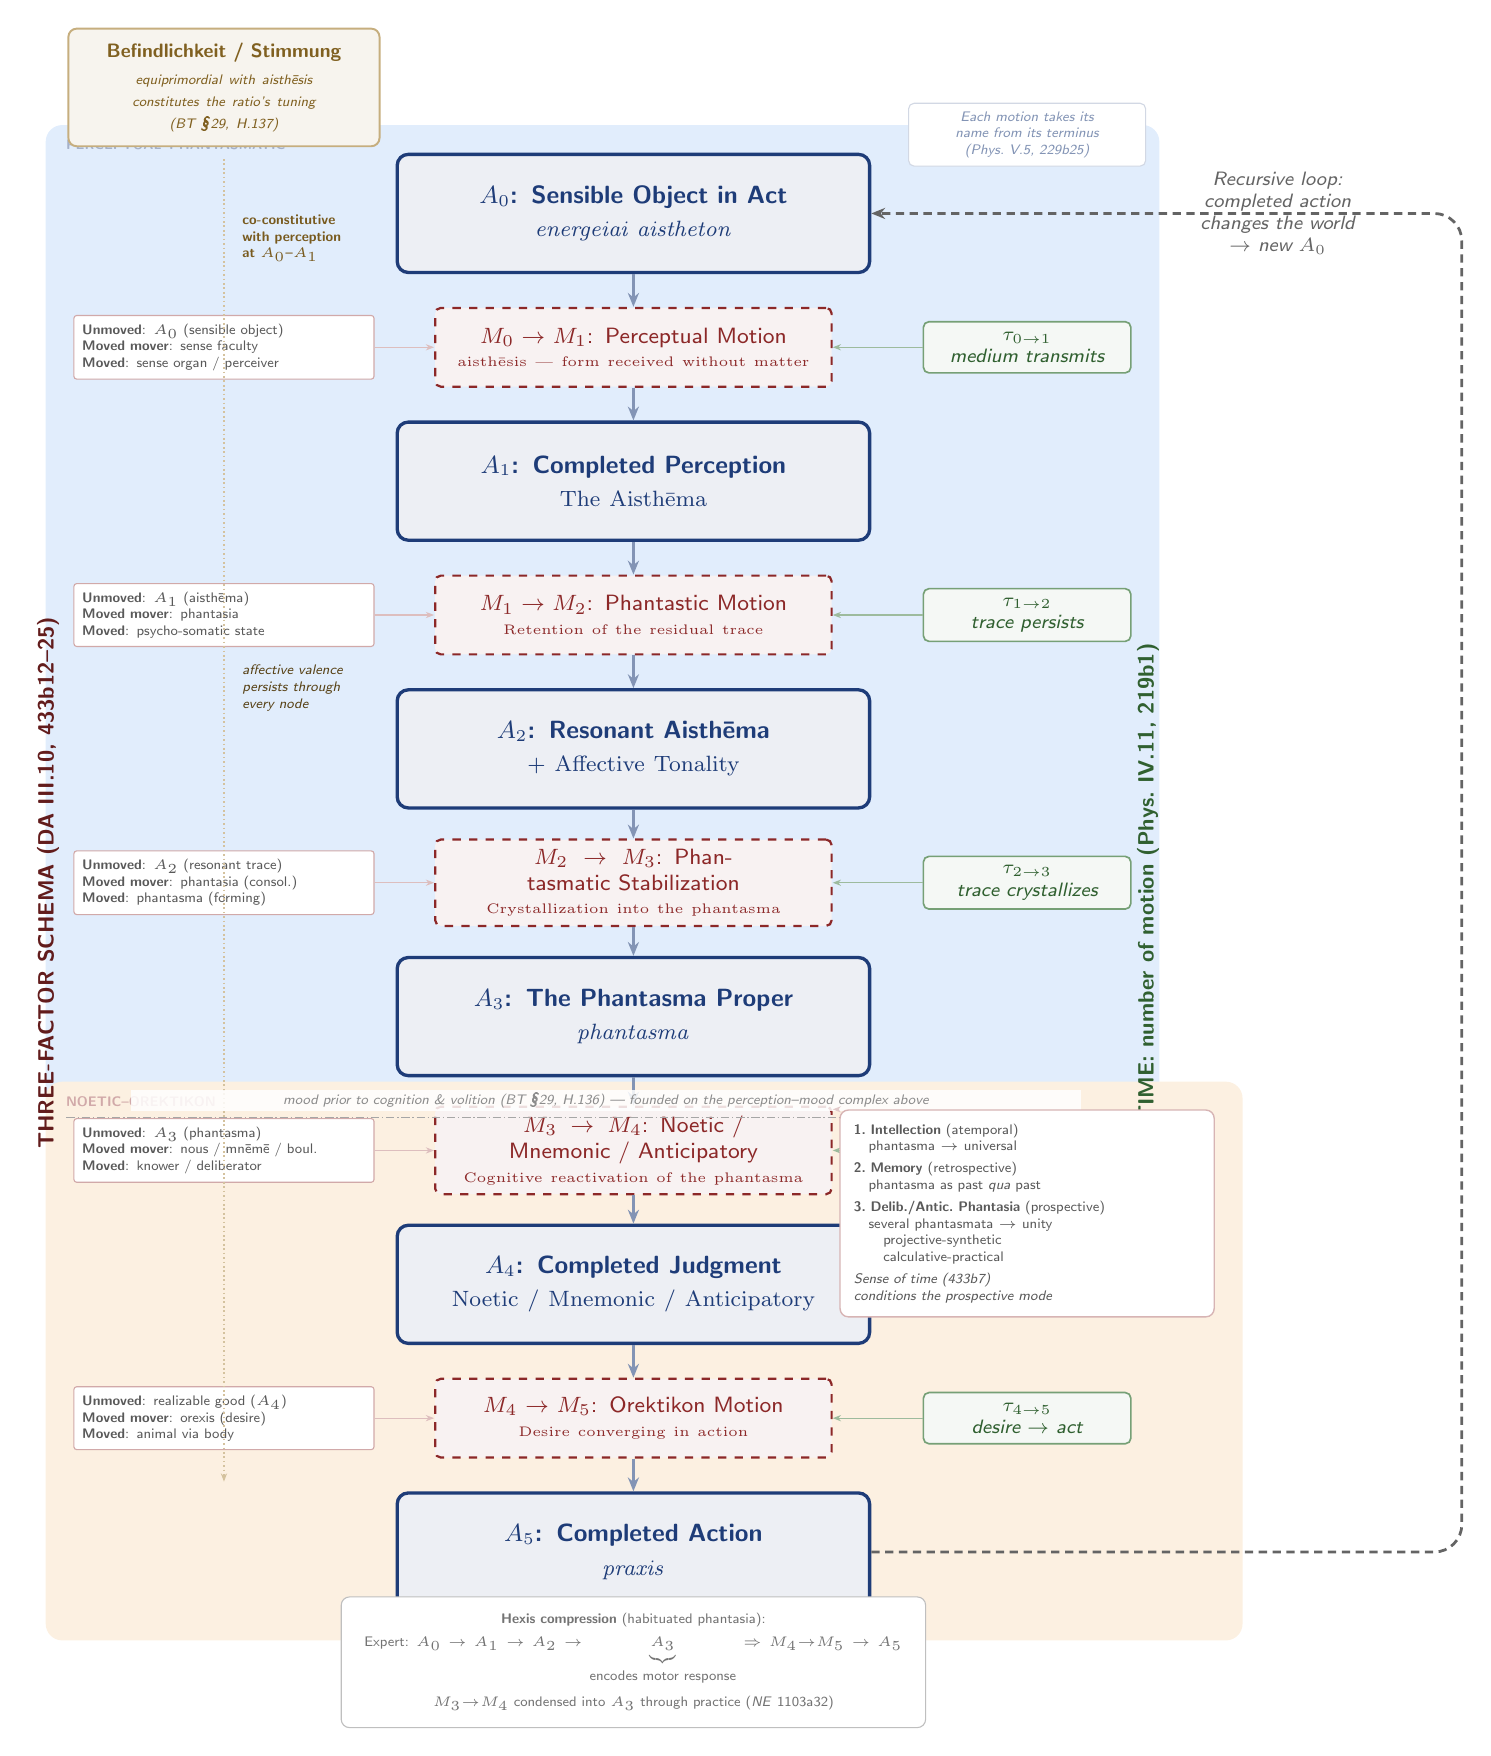
\begin{tikzpicture}[
  actnode/.style={
    rectangle, rounded corners=4pt,
    draw=actuality, fill=actuality!8,
    line width=1.2pt,
    minimum width=6cm, minimum height=1.5cm,
    text width=5.6cm, align=center,
    font=\sffamily\small\bfseries,
    text=actuality
  },
  motionnode/.style={
    rectangle, rounded corners=2pt,
    draw=motion, fill=motion!6,
    line width=0.8pt, dashed,
    minimum width=5cm, minimum height=1cm,
    text width=4.8cm, align=center,
    font=\sffamily\footnotesize,
    text=motion
  },
  timenode/.style={
    rectangle, rounded corners=2pt,
    draw=timecolor!70, fill=timecolor!5,
    line width=0.6pt,
    minimum width=2.6cm, minimum height=0.65cm,
    text width=2.4cm, align=center,
    font=\sffamily\scriptsize\itshape,
    text=timecolor!80!black
  },
  kineticbox/.style={
    rectangle, rounded corners=1pt,
    draw=motion!40, fill=white,
    line width=0.4pt,
    text width=3.6cm, align=left,
    font=\sffamily\tiny,
    text=black!65, inner sep=3pt
  },
  moodnote/.style={
    rectangle, rounded corners=3pt,
    draw=moodcolor!60, fill=moodcolor!8,
    line width=0.7pt,
    text width=3.6cm, align=center,
    font=\sffamily\scriptsize\itshape,
    text=moodcolor!80!black, inner sep=5pt
  },
  chainlink/.style={
    -{Stealth[length=5pt,width=4pt]},
    line width=1.2pt, color=actuality!55
  },
  looparrow/.style={
    -{Stealth[length=5pt,width=4pt]},
    line width=1pt, color=loopcolor, densely dashed
  },
]

% ---- Layout constants ----
\def\nodesep{3.4}
\def\motionoff{1.7}
\def\kinoff{5.2}    % kinetic boxes: distance left of center
\def\timeoff{5.0}   % time boxes: distance right of center

% ============================================================
%  ACTUALITIES (center column)
% ============================================================

\node[actnode] (A0) at (0, 0) {
  $A_0$: Sensible Object in Act\\[1pt]
  {\footnotesize\normalfont\textit{energeiai aistheton}}
};
\node[actnode] (A1) at (0, -\nodesep) {
  $A_1$: Completed Perception\\[1pt]
  {\footnotesize\normalfont The Aisth\=ema}
};
\node[actnode] (A2) at (0, -2*\nodesep) {
  $A_2$: Resonant Aisth\=ema\\[1pt]
  {\footnotesize\normalfont + Affective Tonality}
};
\node[actnode] (A3) at (0, -3*\nodesep) {
  $A_3$: The Phantasma Proper\\[1pt]
  {\footnotesize\normalfont\textit{phantasma}}
};
\node[actnode] (A4) at (0, -4*\nodesep) {
  $A_4$: Completed Judgment\\[1pt]
  {\footnotesize\normalfont Noetic / Mnemonic / Anticipatory}
};
\node[actnode] (A5) at (0, -5*\nodesep) {
  $A_5$: Completed Action\\[1pt]
  {\footnotesize\normalfont\textit{praxis}}
};

% ============================================================
%  MOTIONS (between actualities)
% ============================================================

\node[motionnode] (M01) at (0, -\motionoff) {
  $M_0 \!\to\! M_1$: Perceptual Motion\\[-1pt]
  {\tiny\normalfont aisth\=esis --- form received without matter}
};
\node[motionnode] (M12) at (0, -\nodesep - \motionoff) {
  $M_1 \!\to\! M_2$: Phantastic Motion\\[-1pt]
  {\tiny\normalfont Retention of the residual trace}
};
\node[motionnode] (M23) at (0, -2*\nodesep - \motionoff) {
  $M_2 \!\to\! M_3$: Phantasmatic Stabilization\\[-1pt]
  {\tiny\normalfont Crystallization into the phantasma}
};
\node[motionnode] (M34) at (0, -3*\nodesep - \motionoff) {
  $M_3 \!\to\! M_4$: Noetic / Mnemonic / Anticipatory\\[-1pt]
  {\tiny\normalfont Cognitive reactivation of the phantasma}
};
\node[motionnode] (M45) at (0, -4*\nodesep - \motionoff) {
  $M_4 \!\to\! M_5$: Orektikon Motion\\[-1pt]
  {\tiny\normalfont Desire converging in action}
};

% ============================================================
%  CHAIN ARROWS
% ============================================================

\draw[chainlink] (A0.south) -- (M01.north);
\draw[chainlink] (M01.south) -- (A1.north);
\draw[chainlink] (A1.south) -- (M12.north);
\draw[chainlink] (M12.south) -- (A2.north);
\draw[chainlink] (A2.south) -- (M23.north);
\draw[chainlink] (M23.south) -- (A3.north);
\draw[chainlink] (A3.south) -- (M34.north);
\draw[chainlink] (M34.south) -- (A4.north);
\draw[chainlink] (A4.south) -- (M45.north);
\draw[chainlink] (M45.south) -- (A5.north);

% ============================================================
%  TIME (right column)
% ============================================================

\node[timenode] (T01) at (\timeoff, -\motionoff)               {$\tau_{0 \to 1}$\\medium transmits};
\node[timenode] (T12) at (\timeoff, -\nodesep - \motionoff)    {$\tau_{1 \to 2}$\\trace persists};
\node[timenode] (T23) at (\timeoff, -2*\nodesep - \motionoff)  {$\tau_{2 \to 3}$\\trace crystallizes};
\node[timenode] (T34) at (\timeoff, -3*\nodesep - \motionoff)  {$\tau_{3 \to 4}$\\variable by mode};
\node[timenode] (T45) at (\timeoff, -4*\nodesep - \motionoff)  {$\tau_{4 \to 5}$\\desire $\to$ act};

\foreach \t/\m in {T01/M01, T12/M12, T23/M23, T34/M34, T45/M45} {
  \draw[-{Stealth[length=3pt]}, timecolor!50, thin] (\t.west) -- (\m.east);
}

% Time axis label
\node[timecolor!80!black, font=\sffamily\footnotesize\bfseries, rotate=90, anchor=south]
  at (\timeoff + 1.8, -2.5*\nodesep) {TIME: number of motion (Phys.\ IV.11, 219b1)};

% ============================================================
%  KINETIC ROLES (left column — three-factor schema)
% ============================================================

\node[kineticbox] (K01) at (-\kinoff, -\motionoff) {
  \textbf{Unmoved}: $A_0$ (sensible object)\\
  \textbf{Moved mover}: sense faculty\\
  \textbf{Moved}: sense organ / perceiver
};
\node[kineticbox] (K12) at (-\kinoff, -\nodesep - \motionoff) {
  \textbf{Unmoved}: $A_1$ (aisth\=ema)\\
  \textbf{Moved mover}: phantasia\\
  \textbf{Moved}: psycho-somatic state
};
\node[kineticbox] (K23) at (-\kinoff, -2*\nodesep - \motionoff) {
  \textbf{Unmoved}: $A_2$ (resonant trace)\\
  \textbf{Moved mover}: phantasia (consol.)\\
  \textbf{Moved}: phantasma (forming)
};
\node[kineticbox] (K34) at (-\kinoff, -3*\nodesep - \motionoff) {
  \textbf{Unmoved}: $A_3$ (phantasma)\\
  \textbf{Moved mover}: nous / mn\=em\=e / boul.\\
  \textbf{Moved}: knower / deliberator
};
\node[kineticbox] (K45) at (-\kinoff, -4*\nodesep - \motionoff) {
  \textbf{Unmoved}: realizable good ($A_4$)\\
  \textbf{Moved mover}: orexis (desire)\\
  \textbf{Moved}: animal via body
};

\foreach \k/\m in {K01/M01, K12/M12, K23/M23, K34/M34, K45/M45} {
  \draw[-{Stealth[length=3pt]}, motion!30, thin] (\k.east) -- (\m.west);
}

% Schema label (far left, vertical)
\node[motion!70!black, font=\sffamily\footnotesize\bfseries, rotate=90, anchor=north]
  at (-\kinoff - 2.5, -2.5*\nodesep)
  {THREE-FACTOR SCHEMA (DA III.10, 433b12--25)};

% ============================================================
%  BEFINDLICHKEIT / MOOD (far left, above kinetic column)
% ============================================================

\node[moodnote] (mood) at (-\kinoff, 1.6) {
  \textbf{Befindlichkeit / Stimmung}\\[2pt]
  {\tiny equiprimordial with aisth\=esis}\\
  {\tiny constitutes the ratio's tuning}\\
  {\tiny (BT \S29, H.137)}
};

% Dotted line from Befindlichkeit down the full chain
% with "co-constitutive" label near A0–A1 and "persists" label lower
\draw[moodcolor!45, line width=0.6pt, densely dotted,
  -{Stealth[length=3pt]}]
  ($(mood.south) + (0, -0.15)$) -- ($(K45.south) + (0, -0.4)$)
  node[pos=0.06, right=3pt, font=\sffamily\tiny\bfseries\itshape,
    text=moodcolor!75!black, text width=2.2cm, align=left]
  {co-constitutive\\with perception\\at $A_0$--$A_1$}
  node[pos=0.40, right=3pt, font=\sffamily\tiny\itshape,
    text=moodcolor!55!black, text width=1.8cm, align=left]
  {affective valence\\persists through\\every node};

% ============================================================
%  ONTOLOGICAL PRIORITY LINE
% ============================================================

% Positioned in the gap between A3 bottom and M34 top
% A3 bottom = -3*nodesep - 0.75, M34 top = -3*nodesep - motionoff + 0.5
% midpoint ≈ -3*nodesep - 1.25
\coordinate (divleft) at (-\kinoff - 2.0, -3*\nodesep - 1.28);
\coordinate (divright) at (\timeoff + 1.5, -3*\nodesep - 1.28);

\draw[black!35, line width=0.5pt, densely dash dot]
  (divleft) -- (divright);

\node[font=\sffamily\tiny\itshape, text=black!45,
  text width=12cm, align=center, anchor=south,
  fill=white, fill opacity=0.85, text opacity=1, inner sep=1pt]
  at ($(divleft)!0.5!(divright) + (0, 0.08)$)
  {mood prior to cognition \& volition (BT \S29, H.136) ---
   founded on the perception--mood complex above};

% ============================================================
%  M3→M4 PARALLEL MODES (detail box, right of M34)
%  — defined BEFORE background so 'modes' is available for fit
% ============================================================

\node[rectangle, rounded corners=3pt, draw=motion!35, fill=white,
  line width=0.5pt, text width=4.4cm, align=left,
  font=\sffamily\tiny, text=black!65, inner sep=5pt]
  (modes) at (\timeoff, -3*\nodesep - \motionoff - 0.8) {
  \textbf{1.\ Intellection} (atemporal)\\
  \quad phantasma $\to$ universal\\[2pt]
  \textbf{2.\ Memory} (retrospective)\\
  \quad phantasma as past \textit{qua} past\\[2pt]
  \textbf{3.\ Delib./Antic.\ Phantasia} (prospective)\\
  \quad several phantasmata $\to$ unity\\
  \quad\quad{\tiny projective-synthetic}\\
  \quad\quad{\tiny calculative-practical}\\[2pt]
  {\itshape Sense of time (433b7)\\
  conditions the prospective mode}
};

\draw[-{Stealth[length=3pt]}, motion!25, thin]
  (modes.north west) -- (M34.east |- modes.north west);

% ============================================================
%  BACKGROUND ZONES (after modes is defined)
% ============================================================

\begin{scope}[on background layer]
  % Perceptual-phantasmatic zone (A0–A3)
  \node[fill=perceptual, rounded corners=6pt, inner sep=10pt,
    fit=(A0)(A3)(K01)(K23)(T01)(T23),
    label={[font=\sffamily\tiny\bfseries, text=actuality!40,
      anchor=north west, xshift=4pt, yshift=-2pt]north west:
      PERCEPTUAL--PHANTASMATIC}] (zoneupper) {};

  % Cognitive-practical zone (A4–A5)
  \node[fill=cognitive, rounded corners=6pt, inner sep=10pt,
    fit=(A4)(A5)(K34)(K45)(T34)(T45)(modes),
    label={[font=\sffamily\tiny\bfseries, text=motion!40,
      anchor=north west, xshift=4pt, yshift=-2pt]north west:
      NOETIC--OREKTIKON}] (zonelower) {};
\end{scope}

% ============================================================
%  RECURSIVE LOOP (A5 → A0)
% ============================================================

% Route loop wider to clear the naming principle and time label
\draw[looparrow, rounded corners=10pt]
  (A5.east) -- ++(\timeoff + 2.5, 0)
  -- ++(0, 5*\nodesep)
  -- (A0.east)
  node[pos=0.5, right=5pt, font=\sffamily\scriptsize\itshape,
    text=loopcolor, text width=2.2cm, align=center]
  {Recursive loop:\\completed action\\changes the world\\$\to$ new $A_0$};

% ============================================================
%  NAMING PRINCIPLE (top right annotation)
% ============================================================

\node[rectangle, rounded corners=2pt, draw=actuality!20, fill=white,
  font=\sffamily\tiny\itshape, text=actuality!55,
  text width=2.8cm, align=center, inner sep=3pt]
  at (\timeoff, 1.0) {
  Each motion takes its\\name from its terminus\\
  (Phys.\ V.5, 229b25)
};

% ============================================================
%  HEXIS / COMPRESSION (bottom annotation)
% ============================================================

\node[rectangle, rounded corners=3pt, draw=black!25, fill=white,
  line width=0.4pt, text width=7cm, align=center,
  font=\sffamily\tiny, text=black!55, inner sep=6pt]
  at (0, -5*\nodesep - 1.4) {
  \textbf{Hexis compression} (habituated phantasia):\\[2pt]
  Expert: $A_0 \to A_1 \to A_2 \to
  \underbrace{A_3}_{\text{encodes motor response}}
  \Rightarrow M_4{\to}M_5 \to A_5$\\[3pt]
  $M_3{\to}M_4$ condensed into $A_3$ through practice (\textit{NE} 1103a32)
};

\end{tikzpicture}
\end{document}
